\documentclass[10pt]{report}
\usepackage{listings}
\usepackage{graphicx}
\usepackage{url}

% global commands

\newcommand{\javalst}[2]{
  \lstset{language=Java,captionpos=b,tabsize=4,frame=single,numbers=left,
    numberstyle=\tiny,numbersep=10pt,breaklines=true,showstringspaces=false,
    basicstyle=\footnotesize,emph={label}, caption={#1}, label={#2}}
}
\newcommand{\initlisting}[2]{
  \lstset{language={#1},captionpos=b,tabsize=4,frame=single,numbers=left,
    numberstyle=\tiny,numbersep=10pt,breaklines=true,showstringspaces=false,
    basicstyle=\footnotesize,emph={label}, caption={#2}}
}

\newcommand{\nm}{{\bf proTrade}}
\newcommand{\nmsp}{{\nm \ }}
% end commands
\setlength{\parskip}{0.3cm}
\setlength{\parindent}{0cm}

\begin{document}

\title{\nmsp - A Professional Tennis Trading Environment}

\author{Corina Ciobanu \and Iskander Orazbekov \and Sahin Mir \and Paul Grigoras \and Radu Baltean-Lugojan}

\date{\today}         % inserts today's date

\maketitle            % generates the title from the data above

\begin{abstract}
Tennis trading is a steadily growing market on the Betfair Exchange, with more than 70\% of bets being placed in-play. In order to maintain market liquidity, exchanges must attract customers for example, by supplying them with better tools. By providing more information and better visualization techniques such a tool can help the trader improve his understanding and predict the market evolution, which should (potentially) lead to an increased profit.

In the case of tennis trading, the information required to understand and predict the evolution of the market associated with a particular match consists of the live score, player statistics, potentially a live video feed and - of course - the market data (evolution of betting odds). Ideally, this information is desired for both historical and live matches.

At the moment, no application provides the entire information. A number of solutions exist which allow visualization of historical market data, but they generally lack the more specific, tennis related data. For example the Fracsoft Data Viewer (\cite{site-fracsoft}) does not correlate market data with match data (scores, player statistics). BetAngel (\cite{site-betangel}) provides some tennis related data and prediction, but relies on the user to input the current match score by pushing buttons. This not entirely suited for the high rate with which data is updated. Ideally all the information should be automatically provided to the user to increase update speed and enhance usability.

\nmsp means to fill this gap, by providing all the information, betting and prediction functionalities for both historical and live matches, in an entirely automated fashion.

\end{abstract}

\tableofcontents

\chapter{Introduction}

\section{Importance of Tennis Trading}

This section explains why tennis trading is important, providing background information on the game itself but also on betting and trading.

\subsection{The Game of Tennis }

Many points, short points $\Rightarrow$ high market volatility, ideal for trading.

Tennis is a popular sport played between two players (singles) or between pairs
(doubles). The aim is to win enough points to win a game, enough games to win
a set and enough sets to win a match. Matches are usually played as best of three
sets, but best of five sets are also played in high profile mens tournaments (Grand
Slams). The complex scoring rules lead to a significant number of points being
played in evenly matched games. (Please see Appendix A for the explanation of the Tennis Rules)
An average tennis match lasts between one and two hours and the average num-
ber of points played is about 150. However, late stage matches of a Grand Slam
tournament often last as much as 4-5 hours and many more points are played.


\subsection{Tennis betting}

Tennis betting is the activity of wagering money on a tennis match with the intention of winning additional money.
The pay out on a winning bet is equivalent to the amount betted multiplied by a coefficient called "odds" set by a bookmaker or a 
counterparty.
Tennis betting is largely popular since tournaments are played all around the year
with huge markets being created around every single match, which represents a
major opportunity for profit. It is possible to place bets both before or during
a match (in-play betting). The unpredictable flow of a tennis match makes in-
play betting very exciting as every single point played leads to a change in odds,
especially during the crucial moments of a match where big changes in odds can be
observed. The volatility of odds observed during a tennis match is very similar to
the stock markets, but over a much shorter period of time.
(Please see Appendix B for a brief introduction to betting)


\subsection{Tennis Trading}

Tennis is an ideal trading sport due to the large number of points played and the volatility of odds created
by the unpredictable flow of a tennis match. Professional betters can speculate the large
fluctuation of the betting odds during the matches to obtain profit, regardless of
the match outcome. This is known as tennis trading. (Please see Appendix B for a brief overview of tennis trading and an example of trading).
The following graph represents the trend in the market volume of the tennis betting.

\begin{figure}[ht]
\centering
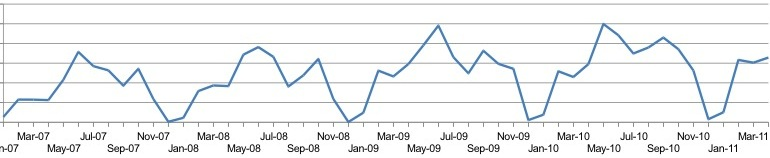
\includegraphics[scale=0.4]{bftennis.jpg}
\caption{}
\end{figure}
\url {http://www.fracsoft.com/index.php?option=com_content&task=view&id=109&Itemid=137}

From the graph above we can clearly observe the market volume is steadiliy increasing year by year and it's peaking at 
Grand Slams tournaments which are the most important tennis events of the year in terms of public attention, ranking points and prize-money awards.
For example, the market created around the US Open Final 2011 had a value of 40 millions which represents the total value of the bets actually matched.
From the total amount of the matched bets, 70 percent are made in-play, meaning that most of the betters are following the odds trend closely for 
speculative purposes. 
There are several factors which have contributed to the increasing popularity of the tennis trading such as:
\begin{itemize}
\item increasing popularity of the game of tennis 
\item increasing worldwide internet access and a faster internet speed  
\item increasing number of tennis trading platforms
\end{itemize}



\section{State of the Art Applications for Tennis Trading}

Although, as we have seen, tennis trading is a major market there are currently no good applications to support it.
Explain why, give examples.

\section{Our Solution}

\nmsp aims to fill this gap by providing ... (Briefly describe functionality, explaining why our application solves the issues $\rightarrow$ answering ``Why should you buy this product?'')

\chapter{Technical Description}

This chapter introduces the main technologies used in building the {\nmsp} application and provides a high level overview of the application's design, describing some of the main technical challenges and how they were overcome.

\section{Technologies}
To facilitate the development of a responsive and feature rich application such as {\nm}, a number of technologies, frameworks and libraries were used throughout the development stage.
This section provides a brief overview of the technologies used while a more in-depth analysis of the choice of technology is presented in section \ref{sec-choice}.

\subsection{Languages}

\begin{description}
\item[Java] This is a widely used multi-purpose programming language, with good support for concurrency. It is platform-independent and provides a choice between native and emulated graphical toolkits.

\item[XML] Usually the langauge of choice for managing the configuration of Java projects, XML is ``typed'' (via schemas) and exstensbile. It is generally used in conjuncture with build automation tools such as Ant.

\item[Bash] Bash scripts are useful for automating simple, repetitive tasks such as builds, pre-commit hooks etc.

\end{description}

\subsection{UI Libraries} 

\begin{description}

\item[SWT] 
SWT is a graphical widget toolkit with a platform dependent implementation. At the heart of its architecure is the ability to create native widgets. However this raises the issue of freeing allocated memory (which cannot be garbage col- lected by the JVM).

``The Standard Widget Toolkit is a graphical widget toolkit for use with the Java platform. It was originally developed by IBM and is now maintained by the Eclipse Foundation in tandem with the Eclipse IDE. It is an alternative to the AWT and Swing Java GUI toolkits provided by Sun Microsystems as part of the Java Platform, Standard Edition.

To display GUI elements, the SWT implementation accesses the native GUI libraries of the operating system using JNI (Java Native Interface) in a manner that is similar to those programs written using operating system-specific APIs. Programs that call SWT are portable, but the implementation of the toolkit, despite part of it being written in Java, is unique for each platform.''

\item[JFace]

\item[SWTChart] The SWTChart API provides a chart component with several basic function-
alities (such as drawing line functions, bar charts etc). The chart can handle
real-time updates (even for large data series), which is crucial to the purpose
of our project and, since it is based on SWT, it integrates smoothly with the
application’s UI design and implementation.

\end{description}


\subsection{Build Automation Tools}

\begin{description}
\item[Apache Ant] is a Java tool used for application builds. It provides out of the box tasks varying from simple file and folder manipulation to compilation and can be extended with more complex tasks such as testing and reporting for applications. These are usually provided by the API developper (e.g. JUnit or Cobertura) simplifying the process of integrating various technologies.

\initlisting{Xml}{An example Ant task for generating PMD reports}
\begin{lstlisting}
<target name="pmd">
	<taskdef name="pmd" classname="net.sourceforge.pmd.ant.PMDTask" classpathref="classpath" />
	<mkdir dir="${pmd.report.dir}" />
	<pmd shortFilenames="true">
		<ruleset>basic,design,braces,junit</ruleset>
        <formatter type="xml" toFile="${pmd.report.dir}/pmd.xml" />
		<fileset dir="${src.dir}">
			<include name="**/*.java" />
		</fileset>
		<fileset dir="${unit.test.dir}">
			<include name="**/*.java" />
		</fileset>
		<fileset dir="${system.test.dir}">
			<include name="**/*.java" />
		</fileset>
	</pmd>
	<xslt in="${pmd.report.dir}/pmd.xml" style="${config.pmd.dir}/format.xslt" out="${pmd.report.dir}/pmd.html" />
	</target>
\end{lstlisting}
\item[make] 
\end{description}

Our choice of technologies is explained in more detail in section ***.

\section{Design}
Explain the design of the software (high-level), possibly including a diagram of the major components of the project.

The diagram can be similar to the one on the slides, but should contain more technical information (not too much).

\section{Achievements/Results}
This section briefly looks at the main achievements and results of the project.
e.g. We delivered an application which does this and that (possible a screenshot could be included).

\chapter{Software Engineering Issues}

This chapter discusses how important aspects of Software Engieering were tackled.

\section{Choice of Technology}
\label{sec-choice}
What technology was used and why? What other technology was considered but not used and why?

(Here we look at the technology options - e.g. SWT vs Swing - and explain our choices.)

\section{Technical Challenges}
Any technical challenges encountered and how addressed?

\section{Risks}
Any risks anticipated, and how mitigated?

\section{Collaboration}
Any collaboration/coordination difficulties encountered and how addressed 

\section{Development Methodologies}
Methods \& Tools

\section{Testing}
Methods \& Tools

\section{Comparison of Plans with Actual Achievements }

\section{Effort}
Present estimates of length of code in each of the components, or any other comparable measure of the effort required.

\section{Contributions}
Summary of each team member's contributions 


\chapter{Validation}
Describes user validation \& testing methods in more detail.
Details of feedback from various groups.

\chapter{Conclusions}
  \begin{itemize} 
  \item Was the project successful?
  \item What did you learn?
  \item What might you have done differently?
  \end{itemize}  

\begin{thebibliography}{9}
\bibitem{bk-testing}
  Steeve Freeman, Nat Pryce,
  \emph{Growing Object-Oriented Software, Guided by Tests}, Addison-Wesley 2010

\bibitem{web-cyccom}
  Robert Chatley's course on Software Engineering Methods
  \url{http://en.wikipedia.org/wiki/Cyclomatic_complexity},
  Imperial College London

\bibitem{bk-aglsam}
  Jonathan Rasmusson,
  \emph{The Agile Samurai},
  Pragmatic Bookshelf,
  October 2010.

\bibitem{bk-aglflh}
  Jeff Langr and Tim Ottinger,
  \emph{Agile in a Flash},
  Pragmatic Bookshelf, 
  January 2011.

\bibitem{web-rbc}
  Robert Chatley's course on Software Engineering Methods
  \url{http://www.doc.ic.ac.uk/~rbc/302/},
  Imperial College London

\bibitem{site-fracsoft}
  Site of Fracsoft, authors of Fracsoft Data Viewer
  \url{http://www.fracsoft.com}

\bibitem{site-betangel}
  Site of BetAngel
  \url{http://www.betangel.com}
  
\bibitem{wiki-swt}
  SWT - Wikipedia
  \url{http://en.wikipedia.org/wiki/Standard_Widget_Toolkit}

\end{thebibliography}

\clearpage
\appendix

\chapter{Tennis Rules}

Tennis is played between two players(single) or between pairs(doubles).
The aim is to win enough points to win a game, enough games to win
a set and enough sets to win a match. Matches are usually played as best of three
sets, but best of five sets are also played in high profile mens tournaments (Grand
Slams). 
The game is played on a court with specific dimensions divided by a net of a specific height.
Opponents stand on opposite sides of the court and players deliver the ball in turn.
The player who delivers the ball is called the server and the player who stands opposite and cross-court from the server
is called the receiver. 
The right to serve or choose the side is decided by a toss of a coin or a racquet.
The half on the player's right side is called the deuce court and the left half is called the advantage court. 
The server shall not serve until the opponent is ready. All even points are played from the deuce court and 
all odd number of points played from the advantage court. The servers are made from the deuce court to the opponent service box
on the deuce court or from advantage court to advantage service box. If the server misses his target twice, he loses the point. 
If the ball hits the net and goes in the correct service box, another serve is granted. If the server steps on the baseline before contact is made, 
the serve is deemed a fault. 

The server always calls his score first. If server wins the first point, he/she gets a score of 15. The score is done like a clock. Love means zero in tennis.
The second point is called 30. The third point is called 45(now-a-days known as 40) and the game is won when the score goes back to love. If the score is 40-40, 
also known as deuce, one side must win by two points. ( Love-15-30-40).

The first player to win 6 games by 2, wins the set. If the score is 5-5, the set is played until someone wins 7 games. If the score is 6-6, a tie-breaker is played.
The tie-breaker is scores by one's rather than (Love-15-30-40). The first one to score 7 points by 2 in the tie-breaker wins the set. If the score is 6-6, one side must win
by two points. 
Usually one needs to win 2 sets to win a match, only at high profile mens tournaments (Grand Slams), a player must win 3 sets. 
If the ball goes into the net, or outside the boundaries of the court, the player who hit that ball loses the point. If the ball hits the net during the point and goes into the opponents court, the ball is in play. A player loses the point if he touches the net, drops his racquet while hitting the ball, bounces the ball over the net, hits a part of the surroundings such as the roof, or a tree, the ball touches him or his partner, he deliberately tries to distract the opponent.
A ball that lands on the line is good.

\url{http://westlake.k12.oh.us/hilliard/whspe/tennis/tennis_rules.htm}

\url{http://assets.usta.com/assets/1/15/ITF%20-%20RoT%202010.pdf}


\chapter{About Betting Odds and Tennis Trading}

Tennis betting is the activity of predicting the outcome of a tennis match by placing a wager.
The pay out on a winning bet is equivalent to the amount betted multiplied by a coefficient called "odds" set by a book-maker or a counterparty.
Usually odds are inversely proportional to the player's chances of winning the match.
It is possible to place a back or a lay bet:
\begin{itemize}
\item Back betting - betting for a certain outcome (placing a back on player X -
betting that player X will win)
\item Lay betting - betting against a certain outcome (placing a lay on player X -
betting that player X will lose)
\end{itemize}

Example: 

Rafael Nadal is playing against Roger Federer and a bookmaker sets the back odds as following:\\
R. Nadal               1.8\\
R. Federer             2.1\\

Better A is backing R. Nadal and places a bet of \pounds10. 
Better B is backing R. Federer and places a bet of \pounds 10.

In case R. Nadal wins the match, the pay outs are as following:\\
Better A has a winning bet and he wins \pounds10 x 1.8 = \pounds18\\
His profit is equal to \pounds8.\\
Better B has lost his bet and his loses are equal to \pounds10. \\

The flow of a tennis match is unpredictable and every single point played leads to a change in odds, 
especially in the crucial moments of a match because it increases or decreases the player's chances of winning the match. 
Betting during a tennis match, also called in-play betting, represents 70 percent of the total amount of bets. Professional betters can 
speculate the large fluctuation of the betting odds during the match to obtain profit. All this happens on a betting exchange, where 
betters are offering their own backing/laying odds. 
Below is the a graph representing the fluctuation of odds during the US Open Final when Rafael Nadal played against Novak Djokovic. 
The graph represents the back odds for N. Djokovic. 

\begin{figure}[ht]
\centering
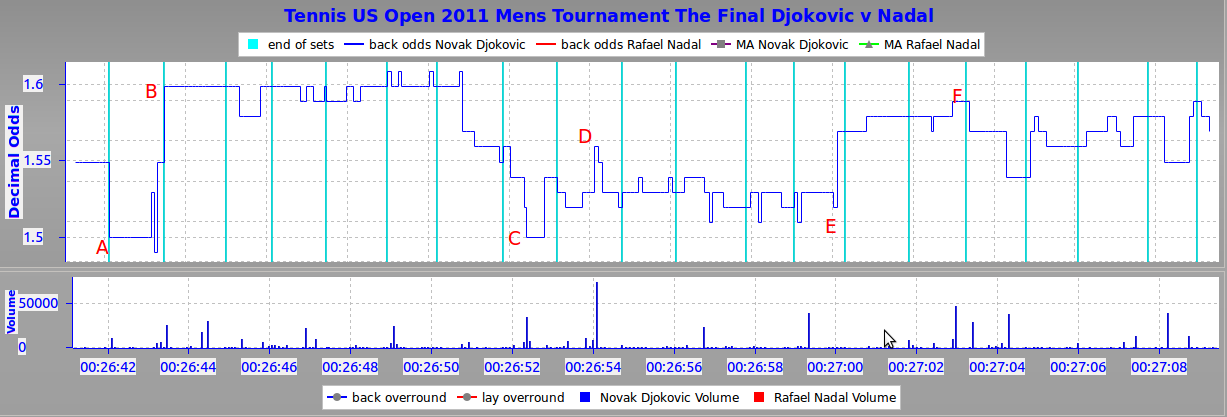
\includegraphics[scale=0.4]{tenistrading.png}
\caption{}
\end{figure}

Now, let's have a look how a professional trader X could make profit from the odds fluctuation during the match.
At point A on the graph, the back odds for N. Djokovic are 1.5. X thinks that the odds are going to grow so he doesn't want to back Djokovic at this point,
instead on the betting exchange he is going to offer to someone else these odds. The offer is accepted by a trader Y who backs Djokovic at 1.5 for a bet of \pounds500. 
At point B, the back odds for N. Djokovic are 1.6. Trader X thinks that the odds are going to fall so he is backing N. Djokovic at 1.6 for a bet of \pounds500. 
He is using the same strategy for points C,D and E,F, so he is offering to someone else odds at points C and E, and is backing at D and F. \\
When the match is over, his bets are as following:\\
Backed N. Djokovic three times at the following odds : 1.6, 1.56,1.58 with a value of each bet of \pounds500. \\
Offered odds to someone else three times at the following values: 1.5,1.5,1.53 with a value of each bet of \pounds500.\\

In case N.Djokovic loses the match, he would lose 3 bets when he backed N. Djokovic but he would win 3 bets because someone else accepted his back odds for N. Djokovic 
and backed N. Djokovic. 
He is losing 3 times \pounds500 but he is winning 3 times back \pounds500, resulting in a P\&L of \pounds0.\\

In case N. Djokovic wins the match, he would win 3 bets when he backed N. Djokovic. \\
His income is going to be: \pounds500 x 1.6+\pounds500 x 1.56+\pounds500 x 1.58 -  \pounds500 x 3 = \pounds870\\
Trader X is going to lose 3 bets because someone else backed N. Djokovic at odds offered by him. \\
His loss is going to be: \pounds500 x 1.5+\pounds500 x 1.5+\pounds500 x 1.53 - \pounds500 x 3  = 765. \\
His final  P\&L in case N. Djokovic wins the match is \pounds870 - \pounds765 = \pounds105

In the tennis trading, professional traders will apply the same strategy as traders in financial markets, Buy Low and Sell High. 

\chapter{User guide}

\section{Installation Instructions}

\section{Quick Start Guide}

\section{FAQ}

\chapter{Exstensive Design}

\chapter{Testing}

\chapter{Statistics}

\chapter{Worklogs}

\end{document}

